%\documentclass[12pt]{article}
%\usepackage{amsmath}
%\usepackage{natbib}
%\usepackage[utf8]{inputenc}
%\usepackage{graphicx}
%\usepackage{subcaption}
%\usepackage{float}
%
%%\usepackage{fancyhdr}
%%\fancyhf{}
%%\fancyhead[R]{\thepage}
%
%
%
% \begin{document}
%% \pagestyle{fancy}
%
%\title{C++ Webserver - APK exam project}
%\author{Mikkel Poulsen, Lars Hjerrild, Søren Holm}
%
%\maketitle
%\thispagestyle{empty}
%
%\newpage
%\tableofcontents
%
%
%\newpage\section{Introduction}
%%
%%
%%Eksempler på figure \ref{fig:coffee}
%%
%%Random citation \citep{DUMMY:1} embeddeed in text.
%%
%%\begin{figure}[h!]
%%	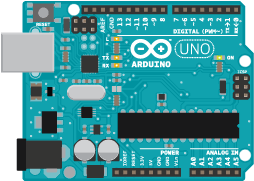
\includegraphics[width=\linewidth]{Figures/Arduino.png}
%%	\caption{Example include.}
%%	\label{fig:examplefig}
%%\end{figure}
%%
%%\begin{figure}[h!]
%%	\centering
%%	\begin{subfigure}[b]{0.4\linewidth}
%%		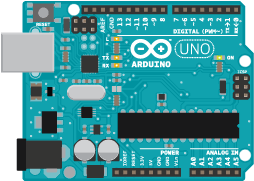
\includegraphics[width=\linewidth]{Figures/Arduino.png}
%%		\caption{Coffee.}
%%	\end{subfigure}
%%	\begin{subfigure}[b]{0.4\linewidth}
%%		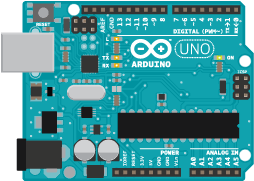
\includegraphics[width=\linewidth]{Figures/Arduino.png}
%%		\caption{More coffee.}
%%	\end{subfigure}
%%	\caption{The same cup of coffee. Two times.}
%%	\label{fig:coffee}
%%\end{figure}\newpage
%%
%% \listoffigures
%% \listoftables
%
% \bibliography{Auto} 
% \bibliographystyle{abbrvnat}
% 
%\end{document}

\documentclass{article}
\usepackage[T1]{fontenc}
\usepackage[utf8]{inputenc}
\usepackage{lmodern}
\usepackage[comma]{natbib}
\usepackage{har2nat}
\usepackage{todonotes}

\bibliographystyle{agsm}
%% or: apsr, dcu, jmr, jphysicsB, kluwer
\usepackage{filecontents}

\begin{filecontents*}{\jobname.bib}
	@incollection{simmons:1980,
		author    = "N. M. Simmons",
		title     = "Behaviour",
		pages     = "124-44",
		year      = 1980,
		booktitle = "The Desert Bighorn",
		editor    = "Gale Monson and Lowell Summer",
		publisher = "University of Arizona Press",
		address   = "Tucson, AZ",
	}
\end{filecontents*}
\begin{document}\pagestyle{empty}
	
	
	
	\title{Anatomi Eksamensprojekt - Fordøjelsessystemet}
	\author{Lars Hjerrild studiednr: 201409555}
	
	\maketitle
	\thispagestyle{empty}
	
	\pagebreak
	\section{Introduction}
	Denne opgave indeholder en anatomisk beskrivelse af de forskellig dele af fordøjelsessystemet. Først vil kirtler og portåresystemet beskrives, og derefter cavitum oris, oesophagus og ventriklen, for til sidst at dykke ned i tarmsystemet.\\
	
	
	\section{Cavitum Oris}
	På dansk hedder cavitum oris mundhulen og er det første led i vores fordøjelses system. Her sker både kemisk og mekanisk nedbrydning af føden. Den kemiske kommer af spyttet der bliver produceret i de tre spytkirtler der hedder GL. sublingulais, Gl. submandibularis og Gl. Parotis.\\ 
	
	Efter at have været igennem munden kommer føden ned igennem pharynx.
	
	\section{Oesophagus}
	Oesophagus som på dansk kaldes spiserøret er et 25 cm langt muskuløst rør, der går fra halsrod til cavitas abdominalis. Undervejs går oesophagus igennem diaphragma ved hiatus oesophagus. I cervix/collum har oesophagus relationer til Gl. thyroidea, trachea og n. Larygeus recurrens \todo{Add more}.\\
	
	Oesophagus løber ligeledes ned igennem thorax hvor den har et andet set af relationer. Posteriort ligger Collumna, og dereter vil man sige at oesophagus havde forskellige relationer ift. hvilken del af mediastinum den lå i.\\
	
	I mediastinum superius ligger Trachea og bifurcaturen anteriort. På højre side ligger pulmones dxt og den dertilhørende pleura, samt v. Azygos. På venstre side af oesophagus ligger a. Carotis cummunis sin, A. Subclavia sin og Argus aorta. Dette er relationerne i medistinum superius.
	
	I medistinum posterius ligger Aorta descendens pars thoracica, Ductus thoracicus og v. Azygos posteriort ift. oesophagus. Der er relationer til begge pulmones og pleura. På venstre side er der ligeledes relation til aorta descendens pars thorcica, og anteriort er der relation til Cor. N. Vagus omspinder i dette område oesophagus som plexus oesophagus.\\
	
	Sidst går oesophagus igennem diaphragma og ender i ventriklens cardia, hvor den anteriort dækkes af Hepa\todo{Look it up}.
	
	 
	 
	\section{Ventriklen}
	Ventriklen eller gastor er det vi på dansk kalder mavesækken. Helt generelt om gastor kan sige at den fungerer som et reservoir for føde. I gastor er der både mekaniske og kemiske mekanismer der hjælper til nedbrydelsen af føde, hvor den kemiske del er saltsyre. Vetriklens placering i abdomen er intraperitonalt, og ellers opad mod venstre i cavitas abdominalis. Ventriklen kan opdeles i 4 dele. 
	\begin{enumerate}
		\item Pars Cardia
		\item Fundus ventriculi
		\item Corpus ventriculi
		\item Pars pulorica
	\end{enumerate}
	Der er åbninger til ventriklen ved Cardia, (hvor oesophagus løb ind) og ved Pylorus, som er udgangen til duodenum. Ved sidstnævnte er der en ringmuskel der kan styrer tømningen. Ventriklen har to kanter som er curvatura minor og curvatura major. 
	
	\subsection{Curvatura minor}
	Dette kaldes den lille kant som er ca. 10 cm lang. \todo{add more}
	\subsection{Curvatura major}
	\todo{add more}
	
	Ventrikler har to krøs som er Ommentum minus et major
	
	\subsection{Ommentum major}
	
	
	Hvis man ser på ventriklen kan struktur indefra og ud kan man opdele det i. \todo{add opdeling}
	
	\subsection{Relationer}
	
	Anteriort har forfladen af ventriklen relationer til Diaphragma og den forreste bugvæg. Derudover desuden også til Hepars underside, og til splen. Som posteriore relationer ligger diagraphma, Renalis sin. og Gl. suprarenalis sin, pancreas, den venstre colofleksur og mesocolen.
	
	Ventriklens kar kommer fra grene fra truncus coeliacus, og venerne følger her arterierne, men udmunder i V. portae.
	
	Lymfen dræneres til ductus thoracicus.
	
	Ventriklen er desuden styret det sympatiske og parasympatiske nervesystem. Sympaticus innerveres\todo{check} af Truncus sympaticus, hvilket hæmmer motorik og aktivere lukkemuskulaturen ved ventriklen. Parasympaticus aktiveres af Nn. Vagi der fremmer sekration og motorik, samt afslapper lukkemuskulaturen. 
	
	
	\section{Intenstinum tenue}
	Efter at have været i ventriklen går maden videre til tyndtarmen der hedder intenstinum tenue. Dette er et 4-6 meter langt muskulært rør, der går fra pyleros til coecum. Så intenstinum tenue forbinder ventriklen med intestinum crassum. Funktionen af tyndtarmen er nedbrydning og absorbtion af fedt, kulhydrat, proteiner, vitaminer, og mineraler. 
	
	Intenstinum tenue kan inddeles i tre sektioner :
	
	\begin{enumerate}
		\item Duodenum
		\item Jejenum
		\item Ileum
	\end{enumerate}
	
	
	\section{Duodenum}
	Duodenum er det vi på dansk kalder for tolvfingertarmen. Denne er ca. 25 cm lang, hvor ca. de første 2 cm er intraperitonaele, og resten er retroperitonealt. Dette betyder også at duodenum ikke har noget krøs. Duodenum kan indeles i fire dele:
	\begin{enumerate}
		\item Pars superior duodeni
		\item Pars descendens duodeni
		\item Pars horisontalis/inferior duodeni
		\item Pars ascendens duodeni
	\end{enumerate}
	
	I Pars descendens findes parpilla duodeni major, som er udmundingen ductus pancreaticus og ductus choledocus. Ligeledes findes her Papilla duodeni minor hvor pancreaticus accesorius udmunder. Duodenum er forsynet kar der er forgreninger til hhv. truncus coeliacus, og a. mesenterica superior. Duodenum bliver dræneret af v. mesenterica sup. der løber videre ud i v. portae.
	
	\section{Jejenum og Ileum}
	
	Denne del af intenstinum tenue går fra duodenum til papilla ilealis. Disse to dele ligger begge intraperitonalt, og har derfor også et krøs der kaldes mesenteriet. Man opdeler de to dele af tarmen således at ca. 2/5 af den orale del, det vil sige fra udmundingen ved duodenum, kaldes jejnum og resten kaldes for ileum. Opdelingen er lavet fordi der er forskel i tarmens opbygning. Jejenum har en tykkere væg og bredere diameter end Ileum, og ligeledes er slimfolderne højere og bredere. Desuden er Jejenum også noget mere karigt. Jejenum er forsynet af kar fra A. mesenterica superior.
	
	
	Generelt bliver intenstinum tenue påvirket af både parasympaticus og sympaticus. Ved sympaticus hæmmes sekration, peristaltik og der sker aktivering af lukkemuskulatur. Ved Parasymaticus stimuleres sekration og peristaltik, og lukkemuskulaturen hæmmes
	
	\section{Intestinum crasum}
	Efter at maden er gået igennem tyndtarmen ender det til sidst ud tyktarmen. Intestinum crasum er 1.5 meter langt og er organet der danner rammen omkring intestium tenue. Funktionen af denne er at absorbere vand og salte, samt deponere fæces. Intestinum crasum kan inddeles i 6 dele.
	
	\begin{enumerate}
		\item Caecum
		\item Colon ascendens
		\item Colon transversum
		\item Colon descendens
		\item Colon sigmoideum
		\item Intestinum rectum 
	\end{enumerate}
	
	\subsection{Caecum}
	På dansk kaldes denne del for blindtarmen, selvom det ikke er den blindtarm man tænker på. Caecum ligger intraperitonalt, og har modtager den terminale del af Ileum, hvor hullet mellem de to hedder ostium ileale, og frembulingen hedder papilla ilialis.
	
	\subsection{Colon ascendens}
	Ligger retroperitonalt
	
	\subsection{Colon transversum}
	Starter ved Flexura coli dxt.og slutter ved flexura coli sin. Denne del af Intestinum crasum ligger intraperitonalt, og har krøset mesocolen transversum. Den ligger i kontakt med forreste bugvæg og under: lever galdeblære, ventrikel, og splen.
	
	\subsection{Colon descendens}
	Ligger retroperitonalt
	
	\pagebreak
	%\citep{simmons:1980}
	\bibliography{\jobname}
\end{document}